\section{React}

In the last day of the third week, we started discussing React, which is an user interface library created by Facebook on JavaScript. I had almost no experience with both React and JavaScript. 

\subsection{MPA and SPA}

% MPA and SPA
We started the discussion with MPA (multiple page applications) and SPA (single page applications), and why SPA should be chosen over MPA. React helps developers to develop SPA by using JavaScript and virtual DOM. Since our main concern will have been learning React, we talked about the advantages and limitations of it, and compared React with other frameworks and libraries by looking at the trends in order to have better perspective.

% Rendering UI
We started with the React elements and continued with the fact that how we can render them. After learning basics, we talked about JSX, which is a syntax extension to JavaScript that allows React elements to be written inside JavaScript using HTML tags. Since JSX many different features such as styling the elements and inserting JavaScript variables, we had to spend a lot of time on it by solving mini coding challanges.

\subsection{Functional and Class Components}

% Functional components and class components
\begin{wrapfigure}{r}{0.3\textwidth}
  \centering
  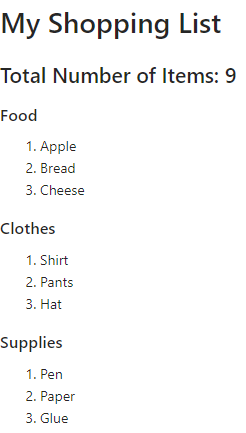
\includegraphics[width=0.3\textwidth]{img/shopping-app.png}
  \caption{Basic Shopping List App}
\end{wrapfigure}
We moved into components. A React component can be defined as an independent reusable component that outputs the React element. We compared the class and functional components and discussed the usage differences of them. I realized that I was tend to use class components because of the OOP and class familarities although functional components are excessively used in the sector.

After these, we solved an example, which can be called Shopping List App. It was a simple shopping list without adding or removing options, but the it only were showing the provided list. After we coded the exercise, out mentor also coded the exercise to show us another prespective.

\subsection{States}

% States
Then we discussed a crucial topic and feature of React, States. We talked what a state is and how we it is used. We then jumped into the another important topic in states: setting/updating the state. We realized and learned how to fix the different behaviours of setting states.

\subsection{Life Cycle Methods}

% Life Cycle Methods
Another essential topic was life cycle methods of class components. While rendering and mounting the component, React runs various methods on the components at multiple phases. Life cycle methods can be used for specific purposes according to phases.

\subsection{Evetn Handlers}

% Event Handlers
Event handling is pretty similar to HTML events. We disccussed taht we can achieved some effects by using event handlers. For example, sending a request when a button is clicked or changing the state of a variable when a key is pressed can be achieved by event handlers.

\subsection{Promises, Back-end Requests and JWT}

% Promises and Backend Request
After the basics and some advanced topic, we moved into the back-end requests. Just before talking about them, we discussed the promises, a feature of JavaScript. For back-end requests, we conversed about axios. Axios provides support to different request types and configs, and it is easy to use.

% JWT
We briefly talked about JWT tokens used for the token based authentication instead of password authentication everytime.





